\section{Results}
\label{sec:results}
\subsection{Frozen source selection against pressure control}
The final comparison comprises 1,344 completed runs across six methods, four scenarios, and 56 paired seeds. The frozen \method\ selector achieves the lowest equal-city mean waiting in Table~\ref{tab:source-selector}. Its registered mean city-wise relative change against MaxPressure is $-2.42\%$, with a paired 95\% interval of $[-4.58,-0.66]\%$. Waiting improves in 40 of 56 equal-city seed means, and the Holm-adjusted Wilcoxon p-value is 0.0058. Jinan improves by 2.10\%, with all 56 seed means favorable and interval $[-2.35,-1.85]\%$ for relative change. Los Angeles improves by 2.74\% on average, with 33 favorable seeds and interval $[-7.05,0.77]\%$.

\begin{table*}[!t]
\caption{Frozen Source Selection: Four Scenarios and 56 Paired Seeds}
\label{tab:source-selector}
\centering
\begin{tabular}{lrrrrr}
\toprule
& \multicolumn{3}{c}{Waiting, all departed vehicles (s)} & System & Demand\\
\cmidrule(lr){2-4}
Controller & Los Angeles & Jinan & Equal-city mean & vehicle-hours & completion\\
\midrule
\method, frozen selector & 201.68 & 89.64 & \textbf{145.66} & 585.42 & 0.895\\
Legacy target anchor & 201.68 & 93.97 & 147.83 & 588.48 & 0.894\\
Equal source weights & 212.45 & 89.62 & 151.03 & 586.27 & 0.895\\
Frozen dense linear residual & 211.73 & 104.59 & 158.16 & 613.28 & 0.876\\
PhasePressure & 231.36 & 89.73 & 160.55 & 600.47 & 0.878\\
MaxPressure & 221.49 & 91.57 & 156.53 & 604.78 & 0.879\\
\bottomrule
\end{tabular}
\vspace{3pt}
\begin{minipage}{\textwidth}\footnotesize
Each row contains 224 complete runs. These are raw equal-city means; registered relative effects first form ratios within each city and seed, then average cities and seeds. MaxPressure is a later fixed-baseline supplement on the same cohort, with all models and execution settings unchanged. The target anchor retains a source prior and is not strictly source-free.
\end{minipage}
\end{table*}

\begin{figure*}[!t]
\centering
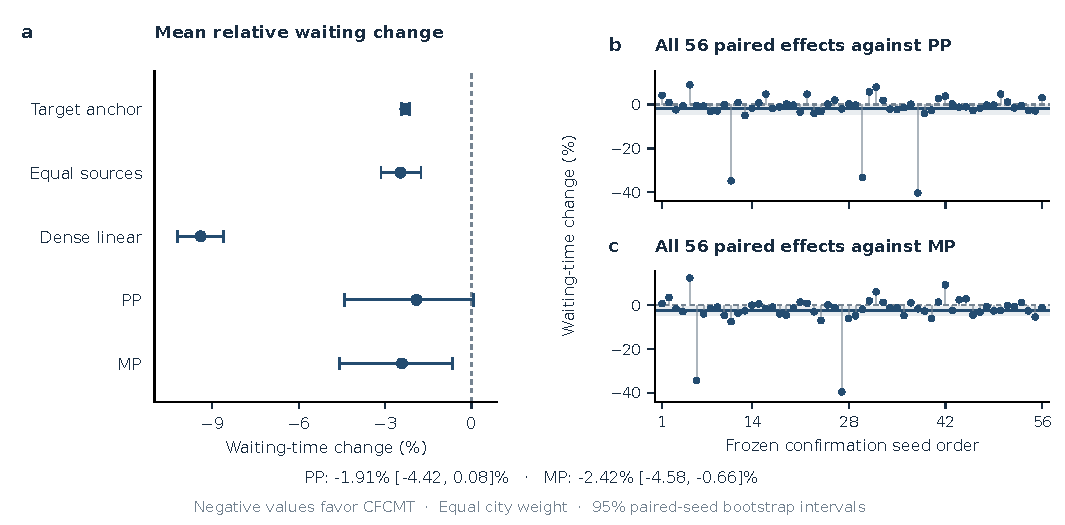
\includegraphics[width=\textwidth]{source_selector_with_mp.pdf}
\caption{Frozen source selection on 56 paired seeds. (a) Mean city-wise relative waiting changes and 95\% paired bootstrap intervals against all five comparators. (b, c) All 56 equal-city relative effects against PhasePressure (PP) and MaxPressure (MP), in the frozen seed order. Solid lines mark means, shaded bands their intervals, and dashed lines zero. Negative values favor the selected controller. Scenarios are averaged within each city before forming relative changes; cities receive equal weight.}
\label{fig:comparisons}
\end{figure*}

Against PhasePressure, the registered mean change is $-1.91\%$, with interval $[-4.42,0.08]\%$ and 34 favorable seed means. The city-specific changes are $-3.73\%$ for Los Angeles and $-0.10\%$ for Jinan. Its equal-city interval crosses zero. Figure~\ref{fig:comparisons} retains all comparator intervals and all 56 seed effects against both pressure rules, including the large favorable tails.

\subsection{Source selection and learned comparators}
Against the legacy target anchor, equal source weights, and the frozen dense linear baseline, the corresponding relative changes are $-2.30\%$, $-2.46\%$, and $-9.40\%$, respectively; all three paired intervals exclude zero. The selected controller exactly matches the target anchor in Los Angeles and improves on it by 4.60\% in Jinan, with all 56 Jinan seed means favorable. The raw equal-city waiting means in Table~\ref{tab:source-selector} and the registered mean relative changes summarize the same complete runs with different weighting: taking a ratio after pooling the waiting values gives greater weight to large Los Angeles values.

Appendix~\ref{app:development-results} reports the earlier models' full offline and closed-loop comparisons, the ten-seed frozen-model confirmation, and the separately selected Jinan controller. Those experiments use different fitted models or selection procedures and are not pooled with the final source selector.
